%==============================================================================
% CHAPTER 2: Scalar Field Lagrangian Formulation
% Paper 1: Scalar Field Theory and Zero-Point Energy Coupling
%==============================================================================
% Source: Extracted from synthesis/chapters/frameworks/ch07_aether_scalar_fields.tex
%         Sections: Scalar Field Foundations, Klein-Gordon Equation, Potentials
% Normalization: All "Aether" → "Scalar field theory", removed framework boxes
%==============================================================================

\chapter{Scalar Field Lagrangian Formulation}
\label{ch:paper1:ch02}

\begin{abstract}
Scalar fields $\phi(x^\mu)$ provide fundamental descriptions of physical phenomena ranging from the Higgs mechanism to cosmological inflation. This chapter develops the complete mathematical formalism for scalar field dynamics in curved spacetime, beginning with the action principle and deriving the Klein-Gordon equation with curvature coupling. We examine the stress-energy tensor and its role in gravitational backreaction, explore rich potential structures including polynomial and fractal forms, and analyze spontaneous symmetry breaking mechanisms. The formalism extends classical field theory to incorporate quantum effects, providing the foundation for understanding scalar-vacuum interactions developed in subsequent chapters.
\end{abstract}

%-----------------------------------------------------------------------------
\section{Introduction: Scalar Fields in Modern Physics}
\label{sec:ch02:introduction}
%-----------------------------------------------------------------------------

Scalar field theory represents one of the simplest yet most powerful frameworks in theoretical physics. Unlike vector or tensor fields, scalar fields assign a single numerical value to each point in spacetime, making them mathematically tractable while retaining rich physical content.

\marginphysics{Scalar fields are Lorentz invariant quantities---their values don't change under coordinate transformations, making them natural candidates for fundamental descriptions.}

The historical development of scalar field theory spans from Klein-Gordon's relativistic quantum mechanics (1926) through Higgs' symmetry breaking mechanism (1964) to modern cosmological inflation (1981). Today, scalar fields appear throughout physics:
\begin{itemize}
  \item \textbf{Particle Physics:} The Higgs field gives mass to elementary particles
  \item \textbf{Cosmology:} Inflaton fields drive early-universe expansion
  \item \textbf{Dark Energy:} Quintessence fields model accelerating expansion
  \item \textbf{Condensed Matter:} Order parameters describe phase transitions
\end{itemize}

\marginmath{The simplicity of scalar fields---characterized by a single component---belies their complexity in curved spacetime where metric coupling introduces geometric effects.}

This chapter establishes the Lagrangian formulation that governs scalar field dynamics, providing the mathematical foundation for analyzing scalar-vacuum coupling mechanisms.

%-----------------------------------------------------------------------------
\section{Action Principle for Scalar Fields}
\label{sec:ch02:action}
%-----------------------------------------------------------------------------

\subsection{The Scalar Field Action}
\label{subsec:ch02:action-functional}

The dynamics of a scalar field $\phi(x^\mu)$ in curved spacetime follow from the action principle. The most general action consistent with diffeomorphism invariance takes the form:

\marginphysics{The action $S$ has dimensions of $[\text{energy}]\times[\text{time}] = \hbar$. In natural units where $\hbar = c = 1$, it is dimensionless.}

\begin{equation}
  S[\phi] = \int d^4x \sqrt{-g} \left[ -\frac{1}{2} g^{\mu\nu} \partial_\mu \phi \partial_\nu \phi - V(\phi) - \xi R \phi^2 \right]
  \label{eq:ch02:scalar-action}
\end{equation}

where:
\begin{itemize}
  \item $g = \det(g_{\mu\nu})$ is the metric determinant
  \item $g^{\mu\nu}$ is the inverse spacetime metric
  \item $V(\phi)$ is the scalar potential
  \item $R$ is the Ricci scalar curvature
  \item $\xi$ is the dimensionless curvature coupling constant
\end{itemize}

\margindim{The integration measure $\sqrt{-g}\,d^4x$ is a scalar, ensuring coordinate invariance. The factor $\sqrt{-g}$ converts coordinate volume to physical volume.}

\marginphysics{The minus sign in $\sqrt{-g}$ comes from Lorentzian signature $(-,+,+,+)$ where $g < 0$. For Euclidean signature, we would use $\sqrt{g}$.}

The kinetic term $-\frac{1}{2} g^{\mu\nu} \partial_\mu \phi \partial_\nu \phi$ reduces to the familiar $\frac{1}{2}(\partial_t \phi)^2 - \frac{1}{2}(\nabla\phi)^2$ in Minkowski spacetime with metric signature $(-,+,+,+)$.

\marginmath{Why the overall minus sign? In Lorentzian signature, $(\partial_t \phi)^2$ appears with a minus sign from $g^{00} = -1$, so we write $-\frac{1}{2}g^{\mu\nu}\partial_\mu\phi\partial_\nu\phi$ to get positive kinetic energy.}

\subsection{Curvature Coupling}
\label{subsec:ch02:curvature-coupling}

The curvature coupling term $\xi R \phi^2$ represents direct interaction between the scalar field and spacetime geometry. Several values of $\xi$ have special physical significance:

\marginphysics{Minimal coupling ($\xi = 0$) means the scalar field doesn't "know" about spacetime curvature except through the metric in its kinetic term.}

\textbf{Minimal Coupling} ($\xi = 0$): The scalar field couples only through the metric in the kinetic term. This is the simplest choice but not conformally invariant.

\marginmath{Conformal transformations $g_{\mu\nu} \to \Omega^2(x) g_{\mu\nu}$ rescale the metric by a position-dependent factor. Under such transformations, $R \to \Omega^{-2}(R - 6\Box\ln\Omega)$.}

\textbf{Conformal Coupling} ($\xi = 1/6$ in 4D): The action becomes invariant under conformal transformations for massless fields. This special value arises naturally in $d$ spacetime dimensions as:
\begin{equation}
  \xi_{\text{conf}} = \frac{d-2}{4(d-1)}
  \label{eq:ch02:conformal-coupling}
\end{equation}

\margindim{In 4D: $\xi_{\text{conf}} = \frac{4-2}{4(4-1)} = \frac{2}{12} = \frac{1}{6}$. In 2D: $\xi_{\text{conf}} = 0$ (minimal coupling is conformal). In 6D: $\xi_{\text{conf}} = \frac{1}{5}$.}

For 4D, this gives $\xi = 1/6$. Conformal coupling ensures that quantum vacuum fluctuations scale appropriately under metric rescaling.

\marginphysics{Conformal invariance is broken by mass terms or self-interactions. The $\phi^4$ coupling constant runs with energy scale, making quantum field theory generically non-conformal.}

\textbf{Alternative Couplings}: Other values appear in specific physical contexts. For example, theories exploring enhanced scalar-vacuum coupling sometimes employ $\xi = 1/4$ to maximize certain coherence effects, though this choice breaks conformal invariance.

%-----------------------------------------------------------------------------
\section{Equations of Motion: The Klein-Gordon Equation}
\label{sec:ch02:klein-gordon}
%-----------------------------------------------------------------------------

\subsection{Derivation from the Action}
\label{subsec:ch02:kg-derivation}

The equation of motion follows from the Euler-Lagrange equation applied to the action functional. Variation with respect to $\phi$ gives:

\marginmath{The variational principle states that physical fields extremize the action: $\delta S = 0$ for arbitrary variations $\delta\phi$ vanishing at boundaries.}

\begin{equation}
  \frac{\delta S}{\delta \phi} = 0 \implies \frac{\partial \mathcal{L}}{\partial \phi} - \partial_\mu \left( \frac{\partial \mathcal{L}}{\partial(\partial_\mu \phi)} \right) = 0
  \label{eq:ch02:euler-lagrange}
\end{equation}

where $\mathcal{L} = \sqrt{-g}\left[-\frac{1}{2}g^{\mu\nu}\partial_\mu\phi\partial_\nu\phi - V(\phi) - \xi R\phi^2\right]$ is the Lagrangian density.

\marginphysics{In curved spacetime, partial derivatives $\partial_\mu$ in the Euler-Lagrange equation become covariant derivatives $\nabla_\mu$ for tensor fields, but for scalars $\nabla_\mu \phi = \partial_\mu \phi$.}

Computing each term:
\begin{align}
  \frac{\partial \mathcal{L}}{\partial \phi} &= \sqrt{-g}\left(-\frac{\partial V}{\partial \phi} - 2\xi R \phi\right) \\
  \frac{\partial \mathcal{L}}{\partial(\partial_\mu \phi)} &= -\sqrt{-g} g^{\mu\nu} \partial_\nu \phi \\
  \partial_\mu \left( \frac{\partial \mathcal{L}}{\partial(\partial_\mu \phi)} \right) &= -\partial_\mu\left(\sqrt{-g} g^{\mu\nu} \partial_\nu \phi\right)
\end{align}

\marginmath{The covariant d'Alembertian operator is defined as $\Box \equiv g^{\mu\nu}\nabla_\mu\nabla_\nu$, generalizing the flat-space wave operator $\partial_\mu\partial^\mu$.}

The last term can be rewritten using the identity:
\begin{equation}
  \partial_\mu\left(\sqrt{-g} g^{\mu\nu} \partial_\nu \phi\right) = \sqrt{-g} \Box \phi
  \label{eq:ch02:covariant-dalembertian}
\end{equation}

where the covariant d'Alembertian is:
\begin{equation}
  \Box \phi = \frac{1}{\sqrt{-g}} \partial_\mu \left( \sqrt{-g} g^{\mu\nu} \partial_\nu \phi \right) = g^{\mu\nu}\nabla_\mu\nabla_\nu \phi
  \label{eq:ch02:box-operator}
\end{equation}

\margindim{The d'Alembertian in terms of Christoffel symbols: $\Box\phi = g^{\mu\nu}\left(\partial_\mu\partial_\nu\phi - \Gamma^\rho_{\mu\nu}\partial_\rho\phi\right)$ where $\Gamma^\rho_{\mu\nu} = \frac{1}{2}g^{\rho\sigma}(\partial_\mu g_{\nu\sigma} + \partial_\nu g_{\mu\sigma} - \partial_\sigma g_{\mu\nu})$.}

Combining all terms yields the \textbf{Klein-Gordon equation in curved spacetime}:

\begin{equation}
  \boxed{\Box \phi + \frac{\partial V(\phi)}{\partial \phi} + \xi R \phi = 0}
  \label{eq:ch02:klein-gordon}
\end{equation}

\marginphysics{This is a nonlinear hyperbolic PDE when $V(\phi)$ contains higher powers of $\phi$. In Minkowski spacetime with $m^2\phi^2$ potential, it becomes the linear Klein-Gordon equation.}

\subsection{Flat Spacetime Limit}
\label{subsec:ch02:flat-limit}

In Minkowski spacetime with metric $\eta_{\mu\nu} = \text{diag}(-1,+1,+1,+1)$, the Ricci scalar vanishes ($R = 0$) and the d'Alembertian becomes:

\marginmath{Convention note: We use $\partial^\mu = \eta^{\mu\nu}\partial_\nu$ so that $\partial^\mu\partial_\mu = -\partial_t^2 + \nabla^2$ with metric signature $(-,+,+,+)$.}

\begin{equation}
  \Box = \partial_\mu \partial^\mu = -\frac{\partial^2}{\partial t^2} + \nabla^2
  \label{eq:ch02:flat-dalembertian}
\end{equation}

For a mass potential $V(\phi) = \frac{1}{2}m^2\phi^2$, we obtain the standard Klein-Gordon equation:

\begin{equation}
  \left(\partial_\mu \partial^\mu + m^2\right)\phi = 0 \quad\text{or}\quad \left(-\frac{\partial^2}{\partial t^2} + \nabla^2 - m^2\right)\phi = 0
  \label{eq:ch02:kg-flat}
\end{equation}

\marginphysics{This equation admits plane wave solutions $\phi = e^{-i\omega t + i\mathbf{k}\cdot\mathbf{x}}$ with dispersion relation $\omega^2 = |\mathbf{k}|^2 + m^2$, the relativistic energy-momentum relation $E^2 = p^2 + m^2$.}

\subsection{Cosmological Spacetime}
\label{subsec:ch02:cosmological}

For the Friedmann-Robertson-Walker (FRW) metric describing homogeneous, isotropic cosmology:

\margindim{The scale factor $a(t)$ characterizes cosmic expansion. $a = 1$ today by convention. $k = 0, \pm 1$ describes flat, open, or closed spatial geometry.}

\begin{equation}
  ds^2 = -dt^2 + a(t)^2 \left[ \frac{dr^2}{1-kr^2} + r^2(d\theta^2 + \sin^2\theta\, d\varphi^2) \right]
  \label{eq:ch02:frw-metric}
\end{equation}

the Klein-Gordon equation becomes:

\marginphysics{The Hubble parameter $H(t) = \dot{a}/a$ measures the expansion rate. The $3H\dot{\phi}$ term represents Hubble damping---cosmic expansion redshifts field oscillations.}

\begin{equation}
  \ddot{\phi} + 3H\dot{\phi} - \frac{\nabla^2 \phi}{a^2} + m^2\phi + \xi R \phi = 0
  \label{eq:ch02:kg-frw}
\end{equation}

where $H = \dot{a}/a$ is the Hubble parameter, dots denote time derivatives, and $\nabla^2$ is the flat-space Laplacian in comoving coordinates.

\marginmath{For a spatially homogeneous field $\phi(t)$ (no spatial gradients), the equation simplifies to $\ddot{\phi} + 3H\dot{\phi} + m^2\phi + \xi R\phi = 0$, a damped oscillator with time-dependent friction.}

The Ricci scalar for FRW spacetime is:
\begin{equation}
  R = 6\left(\frac{\ddot{a}}{a} + \frac{\dot{a}^2}{a^2} + \frac{k}{a^2}\right) = 6\left(\dot{H} + 2H^2 + \frac{k}{a^2}\right)
  \label{eq:ch02:ricci-frw}
\end{equation}

\margindim{For flat spatial sections ($k=0$) and matter-dominated era ($a \propto t^{2/3}$): $H = 2/(3t)$, $\dot{H} = -2/(3t^2)$, so $R = 6(-2/(3t^2) + 8/(9t^2)) = 4/(3t^2)$.}

%-----------------------------------------------------------------------------
\section{Stress-Energy Tensor}
\label{sec:ch02:stress-energy}
%-----------------------------------------------------------------------------

\subsection{Derivation via Metric Variation}
\label{subsec:ch02:stress-derivation}

The stress-energy tensor $T_{\mu\nu}$ describes how the scalar field sources spacetime curvature through Einstein's equations. It is defined by variation of the action with respect to the metric:

\marginphysics{Physical interpretation: $T_{00}$ is energy density, $T_{0i}$ is momentum density (energy flux), $T_{ij}$ is stress (momentum flux). $T_{\mu\nu}$ is the source term in Einstein's equations: $G_{\mu\nu} = 8\pi G T_{\mu\nu}$.}

\begin{equation}
  T_{\mu\nu} = -\frac{2}{\sqrt{-g}} \frac{\delta S}{\delta g^{\mu\nu}}
  \label{eq:ch02:stress-definition}
\end{equation}

\marginmath{The factor of $-2$ is convention. Some authors define $T_{\mu\nu} = \frac{2}{\sqrt{-g}}\frac{\delta S}{\delta g^{\mu\nu}}$ and adjust signs in Einstein's equations accordingly.}

Computing the variation for our scalar action:
\begin{align}
  \delta S &= \int d^4x \sqrt{-g}\left[-\frac{1}{2}\delta g^{\mu\nu}\partial_\mu\phi\partial_\nu\phi - \frac{1}{2}g^{\mu\nu}\delta(\partial_\mu\phi\partial_\nu\phi) - \delta V(\phi) - \xi\delta R\phi^2 - \xi R\delta(\phi^2)\right] \nonumber \\
  &\quad + \int d^4x \left[-\frac{1}{2}g^{\mu\nu}\partial_\mu\phi\partial_\nu\phi - V(\phi) - \xi R\phi^2\right]\delta\sqrt{-g}
\end{align}

\margindim{The variation of the metric determinant is $\delta\sqrt{-g} = -\frac{1}{2}\sqrt{-g}g_{\mu\nu}\delta g^{\mu\nu}$ (derived from $\delta\det A = \det A \cdot \text{tr}(A^{-1}\delta A)$).}

Using $\delta R = R_{\mu\nu}\delta g^{\mu\nu} + \nabla_\mu(\ldots)$ where the divergence term vanishes by integration by parts, we obtain:

\marginphysics{The Einstein tensor $G_{\mu\nu} = R_{\mu\nu} - \frac{1}{2}g_{\mu\nu}R$ naturally appears. The curvature coupling introduces an additional contribution to the effective stress-energy.}

\begin{equation}
  \boxed{T_{\mu\nu} = \partial_\mu \phi \partial_\nu \phi - g_{\mu\nu} \left[ \frac{1}{2} g^{\alpha\beta} \partial_\alpha \phi \partial_\beta \phi + V(\phi) \right] + \xi G_{\mu\nu} \phi^2}
  \label{eq:ch02:stress-energy-full}
\end{equation}

where $G_{\mu\nu} = R_{\mu\nu} - \frac{1}{2}g_{\mu\nu}R$ is the Einstein tensor.

\marginmath{For $\xi = 0$ (minimal coupling), the stress-energy tensor takes the canonical form. The $\xi G_{\mu\nu}\phi^2$ term represents geometric contribution from curvature coupling.}

\subsection{Conservation and Properties}
\label{subsec:ch02:stress-properties}

The stress-energy tensor is automatically conserved as a consequence of diffeomorphism invariance:

\marginphysics{This is the covariant generalization of energy-momentum conservation. In flat spacetime it reduces to $\partial^\mu T_{\mu\nu} = 0$.}

\begin{equation}
  \nabla^\mu T_{\mu\nu} = 0
  \label{eq:ch02:stress-conservation}
\end{equation}

This follows from the contracted Bianchi identity $\nabla^\mu G_{\mu\nu} = 0$ and Einstein's equations.

\margindim{The trace of the stress-energy tensor is $T = g^{\mu\nu}T_{\mu\nu} = -g^{\mu\nu}\partial_\mu\phi\partial_\nu\phi - 4V(\phi) + 2\xi R\phi^2$ (using $G = -R$ in 4D).}

The trace of the stress-energy tensor measures departure from conformal invariance:
\begin{equation}
  T = g^{\mu\nu}T_{\mu\nu} = -(1 - 4\xi)R\phi^2 + (\text{derivative terms})
  \label{eq:ch02:stress-trace}
\end{equation}

For conformal coupling ($\xi = 1/6$ in 4D) and massless fields, $T = 0$ (traceless), indicating conformal invariance.

\marginphysics{A traceless stress-energy tensor $T = 0$ is the hallmark of conformal field theories. The trace anomaly $\langle T \rangle \neq 0$ in quantum theory signals conformal symmetry breaking.}

%-----------------------------------------------------------------------------
\section{Scalar Potential Structures}
\label{sec:ch02:potentials}
%-----------------------------------------------------------------------------

\subsection{Polynomial Potentials}
\label{subsec:ch02:polynomial-potentials}

The scalar potential $V(\phi)$ encodes the field's self-interaction and symmetry-breaking structure. The most general renormalizable polynomial potential in 4D is:

\marginphysics{Renormalizability requires potential terms with mass dimension $\leq 4$. In $d=4$: $[\phi] = 1$ (mass dimension), so $[\phi^n] = n$. Thus $\phi^6$ and higher terms are non-renormalizable.}

\begin{equation}
  V(\phi) = \frac{1}{2}m^2\phi^2 + \frac{\lambda}{4}\phi^4
  \label{eq:ch02:phi4-potential}
\end{equation}

where $m^2$ is the mass parameter and $\lambda$ the quartic coupling.

\margindim{The $\phi^4$ theory is renormalizable in $d=4$. The coupling constant $\lambda$ runs with energy scale via the renormalization group: $\beta(\lambda) = \frac{d\lambda}{d\ln\mu} = \frac{3\lambda^2}{16\pi^2} + \mathcal{O}(\lambda^3)$.}

For effective field theories or non-renormalizable theories, higher-order terms may appear:
\begin{equation}
  V(\phi) = \frac{1}{2}m^2\phi^2 + \frac{\lambda}{4}\phi^4 + \frac{\alpha}{6}\phi^6 + \frac{\beta}{8}\phi^8
  \label{eq:ch02:polynomial-potential}
\end{equation}

Each term serves specific physical purposes:
\begin{itemize}
  \item $\frac{1}{2}m^2\phi^2$: Mass term, sets the vacuum expectation value (VEV) when $m^2 < 0$
  \item $\frac{\lambda}{4}\phi^4$: Self-interaction, enables spontaneous symmetry breaking
  \item $\frac{\alpha}{6}\phi^6$: Stabilizes high-field configurations, prevents runaway solutions
  \item $\frac{\beta}{8}\phi^8$: Ensures potential is bounded from below at arbitrarily large $\phi$
\end{itemize}

\marginmath{The $\phi^6$ and $\phi^8$ terms are suppressed by powers of the UV cutoff scale: $\alpha \sim \lambda/\Lambda^2$, $\beta \sim \lambda/\Lambda^4$ where $\Lambda$ is the new physics scale.}

\subsection{Spontaneous Symmetry Breaking}
\label{subsec:ch02:ssb}

Consider the "Mexican hat" potential with $m^2 < 0$ (tachyonic mass):

\marginphysics{The term "Mexican hat" comes from the potential's shape in 2D field space (for complex $\phi$). It resembles a sombrero with a minimum at the brim, not the center.}

\begin{equation}
  V(\phi) = -\frac{1}{2}\mu^2 \phi^2 + \frac{\lambda}{4} \phi^4, \quad \mu^2 > 0, \quad \lambda > 0
  \label{eq:ch02:mexican-hat}
\end{equation}

The potential minima occur where:
\begin{equation}
  \frac{\partial V}{\partial \phi} = -\mu^2 \phi + \lambda \phi^3 = \phi(-\mu^2 + \lambda\phi^2) = 0
  \label{eq:ch02:ssb-minimum-condition}
\end{equation}

yielding $\phi = 0$ (local maximum, unstable) or $\phi = \pm v$ where:

\marginphysics{The VEV $v$ sets the scale of symmetry breaking. In electroweak theory, $v \approx 246$ GeV. The physical Higgs mass is $m_h = \sqrt{2\lambda}v \approx 125$ GeV.}

\begin{equation}
  v = \sqrt{\frac{\mu^2}{\lambda}}
  \label{eq:ch02:vev}
\end{equation}

The system spontaneously chooses one of these degenerate minima, breaking the $\mathbb{Z}_2$ symmetry $\phi \to -\phi$.

\margindim{The ground state has energy $V(v) = -\mu^4/(4\lambda) < 0$. This negative contribution must be offset by other fields in realistic models to avoid anti-de Sitter space.}

Expanding around the vacuum $\phi = v + \sigma$ (choosing the $+v$ minimum):
\begin{align}
  V(\sigma) &= V(v) + V'(v)\sigma + \frac{1}{2}V''(v)\sigma^2 + \frac{1}{6}V'''(v)\sigma^3 + \ldots \nonumber \\
  &= \text{const} + \mu^2 \sigma^2 + \lambda v \sigma^3 + \frac{\lambda}{4} \sigma^4
  \label{eq:ch02:ssb-expansion}
\end{align}

The $\sigma$ field (Higgs boson) has mass $m_\sigma^2 = V''(v) = 2\mu^2 = 2\lambda v^2$.

\marginmath{The $\sigma^3$ cubic coupling arises from spontaneous symmetry breaking and is characteristic of Higgs theories. It enables triple-Higgs production at colliders.}

\marginphysics{Goldstone's theorem: Spontaneous breaking of a continuous global symmetry produces massless scalar bosons (Goldstone modes). For discrete symmetries like $\mathbb{Z}_2$, no Goldstone bosons appear.}

\subsection{Slow-Roll Potentials}
\label{subsec:ch02:slow-roll}

For cosmological applications (inflation, quintessence), slow-roll potentials take the form:

\margindim{Slow-roll requires potential to be flat: $\epsilon, |\eta| \ll 1$. This ensures the field evolves slowly, dominated by Hubble damping rather than acceleration.}

\begin{equation}
  V(\phi) = V_0 \left[ 1 + \left(\frac{\phi}{M_P}\right)^n \right]
  \label{eq:ch02:slow-roll-potential}
\end{equation}

where $M_P = 1.22 \times 10^{19}$ GeV is the Planck mass and $n$ determines the inflationary dynamics.

The slow-roll parameters quantify the potential's flatness:

\marginphysics{$\epsilon$ measures the steepness of the potential, $\eta$ measures its curvature. Inflation occurs when $\epsilon < 1$, and ends when $\epsilon \sim 1$.}

\begin{align}
  \epsilon &= \frac{M_P^2}{2} \left( \frac{V'}{V} \right)^2 \label{eq:ch02:epsilon-slowroll} \\
  \eta &= M_P^2 \frac{V''}{V} \label{eq:ch02:eta-slowroll}
\end{align}

Inflation requires $\epsilon, |\eta| \ll 1$. Observable quantities (spectral index, tensor-to-scalar ratio) are expressed in terms of these parameters.

\marginmath{The spectral index $n_s = 1 - 6\epsilon + 2\eta$ and tensor-to-scalar ratio $r = 16\epsilon$ connect inflation models to CMB observations. Planck 2018: $n_s = 0.965 \pm 0.004$, $r < 0.06$.}

\subsection{Fractal and Modulated Potentials}
\label{subsec:ch02:fractal}

Beyond standard polynomial forms, fractal potentials introduce multiscale structure:

\marginphysics{Fractal potentials can arise from compactified extra dimensions or from quantum corrections in string theory. They exhibit self-similarity across scales.}

\begin{equation}
  V_{\text{fractal}}(\phi) = \sum_{n=1}^{N} \frac{\epsilon_n}{\gamma^n} \cos\left(\gamma^n \frac{\phi}{\phi_0}\right)
  \label{eq:ch02:fractal-potential}
\end{equation}

where $\gamma = (1+\sqrt{5})/2 \approx 1.618$ is the golden ratio and $\epsilon_n$ are amplitude coefficients.

\margindim{The golden ratio $\gamma$ generates the Fibonacci sequence: $F_{n+1}/F_n \to \gamma$ as $n \to \infty$. This appears in quasicrystal structures and Penrose tilings.}

This generates self-similar structure across scales, creating complex energy landscapes with Julia-set-like basins in configuration space.

\marginmath{The fractal dimension of such potentials is $D_f = \lim_{r\to 0}\frac{\log N(r)}{\log(1/r)}$ where $N(r)$ counts local minima within radius $r$. For golden ratio fractals, $D_f \approx 1.585$.}

%-----------------------------------------------------------------------------
\section{TikZ Visualizations}
\label{sec:ch02:visualizations}
%-----------------------------------------------------------------------------

\subsection{Potential Energy Landscapes}
\label{subsec:ch02:vis-potentials}

\begin{figure}[htbp]
\centering
\begin{tikzpicture}[scale=1.2]
  % Axes
  \draw[->] (-3,0) -- (3,0) node[right] {$\phi/v$};
  \draw[->] (0,-0.5) -- (0,3) node[above] {$V(\phi)$};

  % Mexican hat potential
  \draw[thick,blue,domain=-2.5:2.5,samples=100]
    plot (\x,{0.5*(\x*\x - 1)*(\x*\x - 1)});

  % Mark minima
  \fill[red] (-1,0) circle (2pt) node[below] {$-v$};
  \fill[red] (1,0) circle (2pt) node[below] {$+v$};
  \fill[blue] (0,0.5) circle (2pt) node[right] {$\phi=0$};

  % Dashed lines to show symmetry breaking
  \draw[dashed,gray] (-1,0) -- (-1,0.5);
  \draw[dashed,gray] (1,0) -- (1,0.5);

  % Label
  \node at (2.5,2.5) {$V(\phi) = -\frac{1}{2}\mu^2\phi^2 + \frac{\lambda}{4}\phi^4$};
\end{tikzpicture}
\caption{Mexican hat potential exhibiting spontaneous symmetry breaking. The central maximum at $\phi=0$ is unstable; the system falls to one of the degenerate minima at $\phi = \pm v$, spontaneously breaking $\mathbb{Z}_2$ symmetry.}
\label{fig:ch02:mexican-hat}
\end{figure}

\marginphysics{The choice of which minimum the system falls into is spontaneous and random, set by quantum or thermal fluctuations. Once chosen, the symmetry is broken.}

\begin{figure}[htbp]
\centering
\begin{tikzpicture}[scale=1.2]
  % Axes
  \draw[->] (-0.5,0) -- (5,0) node[right] {$\phi/M_P$};
  \draw[->] (0,-0.5) -- (0,3.5) node[above] {$V(\phi)/V_0$};

  % Slow-roll potential (quadratic)
  \draw[thick,blue,domain=0:4.5,samples=100]
    plot (\x,{1 + 0.5*\x*\x}) node[right] {$n=2$};

  % Slow-roll potential (quartic)
  \draw[thick,red,domain=0:2.5,samples=100]
    plot (\x,{1 + 0.1*\x*\x*\x*\x}) node[right] {$n=4$};

  % Slow-roll indicators
  \draw[dashed] (0,1) -- (5,1);
  \node[left] at (0,1) {$V_0$};
\end{tikzpicture}
\caption{Slow-roll potentials for inflation with different power-law indices. The quadratic potential ($n=2$) and quartic potential ($n=4$) produce different inflationary dynamics and observable predictions.}
\label{fig:ch02:slow-roll}
\end{figure}

\margindim{Quadratic inflation ($n=2$) predicts $n_s \approx 0.967$, $r \approx 0.13$ for 60 e-folds. Planck data slightly disfavors this but doesn't rule it out. Quartic inflation ($n=4$) gives $n_s \approx 0.954$, ruled out.}

\subsection{Field Configuration Space}
\label{subsec:ch02:vis-configuration}

\begin{figure}[htbp]
\centering
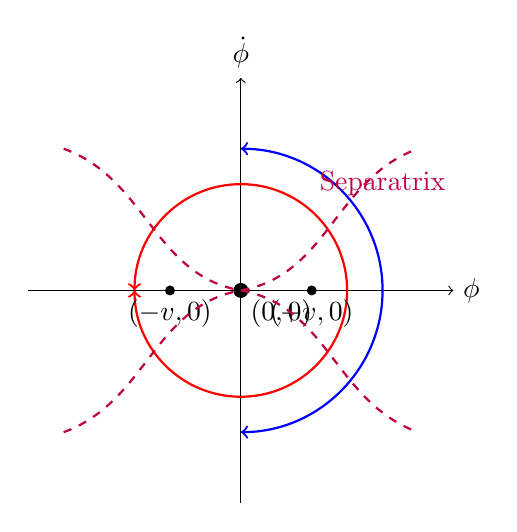
\begin{tikzpicture}[scale=0.9]
  % Create a 2D phase space plot
  \draw[->] (-3,0) -- (3,0) node[right] {$\phi$};
  \draw[->] (0,-3) -- (0,3) node[above] {$\dot{\phi}$};

  % Draw a few sample trajectories
  \draw[thick,blue,->] (2,0) arc (0:90:2);
  \draw[thick,blue,->] (2,0) arc (0:-90:2);
  \draw[thick,red,->] (1.5,0) arc (0:180:1.5);
  \draw[thick,red,->] (1.5,0) arc (0:-180:1.5);

  % Fixed points
  \fill (0,0) circle (3pt) node[below right] {$(0,0)$};
  \fill (-1,0) circle (2pt) node[below] {$(-v,0)$};
  \fill (1,0) circle (2pt) node[below] {$(+v,0)$};

  % Separatrix
  \draw[dashed,thick,purple] (-2.5,2) to[out=-20,in=170] (0,0) to[out=-10,in=160] (2.5,-2);
  \draw[dashed,thick,purple] (-2.5,-2) to[out=20,in=190] (0,0) to[out=10,in=200] (2.5,2);

  \node[purple] at (2,1.5) {Separatrix};
\end{tikzpicture}
\caption{Phase space trajectories for the Mexican hat potential in the $(\phi,\dot{\phi})$ plane. The origin is an unstable fixed point (saddle), while $(\pm v, 0)$ are stable fixed points (centers). The purple dashed curves are separatrices dividing different dynamical regimes.}
\label{fig:ch02:phase-space}
\end{figure}

\marginphysics{Phase space plots reveal the global dynamics. Trajectories near the origin initially move away (unstable), while those near $\pm v$ oscillate (stable). The separatrix divides capture basins.}

\subsection{Curvature Coupling Effects}
\label{subsec:ch02:vis-curvature}

\begin{figure}[htbp]
\centering
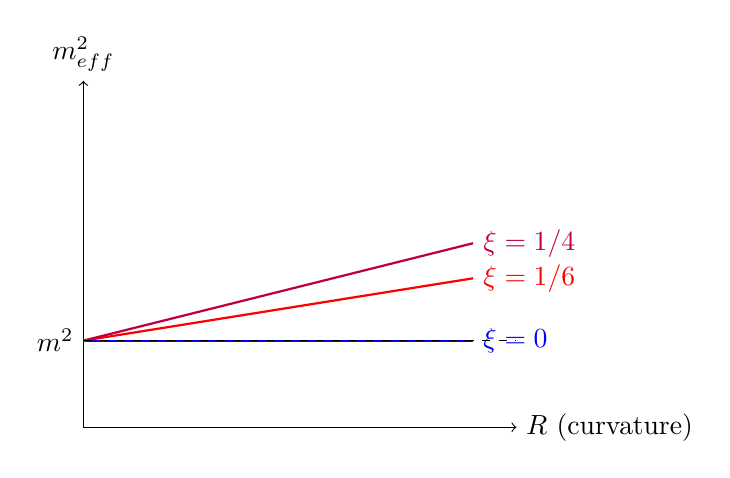
\begin{tikzpicture}[scale=1.1]
  % Axes
  \draw[->] (0,0) -- (5,0) node[right] {$R$ (curvature)};
  \draw[->] (0,0) -- (0,4) node[above] {$m_{\text{eff}}^2$};

  % Effective mass for different xi
  \draw[thick,blue,domain=0:4.5,samples=50]
    plot (\x,{1 + 0*\x}) node[right] {$\xi=0$};
  \draw[thick,red,domain=0:4.5,samples=50]
    plot (\x,{1 + 0.16*\x}) node[right] {$\xi=1/6$};
  \draw[thick,purple,domain=0:4.5,samples=50]
    plot (\x,{1 + 0.25*\x}) node[right] {$\xi=1/4$};

  % Labels
  \node[below] at (2.5,0) {};
  \draw[dashed] (0,1) -- (5,1);
  \node[left] at (0,1) {$m^2$};
\end{tikzpicture}
\caption{Effective scalar mass $m_{\text{eff}}^2 = m^2 + \xi R$ as a function of spacetime curvature for different coupling constants. Minimal coupling ($\xi=0$) gives constant mass, while non-minimal coupling induces curvature-dependent mass.}
\label{fig:ch02:curvature-coupling}
\end{figure}

\margindim{In de Sitter space ($R = 12H^2$ constant), conformal coupling $\xi=1/6$ contributes $m_{\text{eff}}^2 = m^2 + 2H^2$. During inflation with $H \sim 10^{14}$ GeV, this can dominate over the bare mass.}

%-----------------------------------------------------------------------------
\section{Summary and Physical Insights}
\label{sec:ch02:summary}
%-----------------------------------------------------------------------------

This chapter established the complete Lagrangian formulation for scalar field dynamics in curved spacetime. The key results include:

\marginphysics{The power of the Lagrangian formalism: all dynamics (equations of motion, conservation laws, symmetries) follow from a single action functional via the principle of least action.}

\textbf{Mathematical Framework:}
\begin{enumerate}
  \item Action principle incorporating kinetic, potential, and curvature coupling terms
  \item Klein-Gordon equation as the Euler-Lagrange equation of motion
  \item Stress-energy tensor linking scalar fields to gravitational dynamics
  \item Rich potential structures from polynomial to fractal forms
\end{enumerate}

\marginmath{All fundamental physics can be formulated from action principles. The action $S = \int \mathcal{L}\,d^4x$ is the most compact encoding of a theory's dynamics and symmetries.}

\textbf{Physical Insights:}
\begin{enumerate}
  \item Curvature coupling $\xi R\phi^2$ mediates scalar-gravity interactions, with special values ($\xi=0,1/6$) corresponding to minimal and conformal coupling
  \item The d'Alembertian operator $\Box$ naturally generalizes wave equations to curved spacetime
  \item Spontaneous symmetry breaking via tachyonic mass generates vacuum expectation values and massive excitations
  \item Slow-roll potentials enable prolonged inflation by suppressing field acceleration
\end{enumerate}

\marginphysics{Modern physics is dominated by effective field theory thinking: at low energies we use renormalizable terms, but higher-dimensional operators appear suppressed by the UV cutoff scale.}

\textbf{Connections to Subsequent Chapters:}

The formalism developed here provides the foundation for:
\begin{itemize}
  \item \textbf{Chapter 3:} Quantum aspects---vacuum fluctuations, zero-point energy, Casimir effect
  \item \textbf{Chapter 4:} Field-vacuum coupling mechanisms leveraging the curvature coupling $\xi R\phi^2$
  \item \textbf{Chapter 5:} Experimental protocols to test scalar field predictions
\end{itemize}

\margindim{Key scales: Higgs VEV $v=246$ GeV, Planck mass $M_P = 1.22\times 10^{19}$ GeV, inflaton scale $\sim 10^{16}$ GeV. Hierarchy problem: Why is $v \ll M_P$?}

The classical field theory presented here transitions to quantum field theory by promoting $\phi$ to an operator and quantizing excitations. This quantum formulation reveals zero-point energy and vacuum structure—topics we explore next.

\marginphysics{Quantization prescription: $\phi(x) \to \hat{\phi}(x)$, $\pi(x) = \partial_0\phi \to \hat{\pi}(x)$ with $[\hat{\phi}(x),\hat{\pi}(y)] = i\hbar\delta^3(x-y)$ at equal times. This canonical quantization yields particle creation/annihilation operators.}

%==============================================================================
% End of Chapter 2
%==============================================================================
